\documentclass[12pt,a4paper,bibliography=totocnumbered,listof=totocnumbered]{scrartcl}
\usepackage[ngerman]{babel}
\usepackage[utf8]{inputenc}
\usepackage{amsmath}
\usepackage{amsfonts}
\usepackage{amssymb}
\usepackage{graphicx}
\usepackage{fancyhdr}
\usepackage{tabularx}
\usepackage{geometry}
\usepackage{setspace}
\usepackage[right]{eurosym}
\usepackage[printonlyused]{acronym}
\usepackage{subfig}
\usepackage{floatflt}
\usepackage[usenames,dvipsnames]{color}
\usepackage{colortbl}
\usepackage{paralist}
\usepackage{array}
\usepackage{titlesec}
\usepackage{parskip}
\usepackage[right]{eurosym}
\usepackage{picins}
\usepackage[subfigure,titles]{tocloft}
\usepackage[pdfpagelabels=true]{hyperref}

\usepackage{listings}
\lstset{basicstyle=\footnotesize, captionpos=b, breaklines=true, showstringspaces=false, tabsize=2, frame=lines, numbers=left, numberstyle=\tiny, xleftmargin=2em, framexleftmargin=2em}
\makeatletter
\def\l@lstlisting#1#2{\@dottedtocline{1}{0em}{1em}{\hspace{1,5em} Lst. #1}{#2}}
\makeatother

\geometry{a4paper, top=27mm, left=30mm, right=20mm, bottom=35mm, headsep=10mm, footskip=12mm}

\hypersetup{unicode=false, pdftoolbar=true, pdfmenubar=true, pdffitwindow=false, pdfstartview={HSHN},
	pdftitle={Seminar Unternehmensanwendungen},
	pdfauthor={Vedad Hamamdzic},
	pdfsubject={Seminar},
	pdfcreator={\LaTeX\ with package \flqq hyperref\frqq},
	pdfproducer={pdfTeX \the\pdftexversion.\pdftexrevision},
	pdfkeywords={Seminar},
	pdfnewwindow=true,
	colorlinks=true,linkcolor=black,citecolor=black,filecolor=magenta,urlcolor=black}
\pdfinfo{/CreationDate (D:20110620133321)}

\begin{document}

\titlespacing{\section}{0pt}{12pt plus 4pt minus 2pt}{-6pt plus 2pt minus 2pt}

% Kopf- und Fusszeile
\renewcommand{\sectionmark}[1]{\markright{#1}}
\renewcommand{\leftmark}{\rightmark}
\pagestyle{fancy}
\lhead{}
\chead{}
\rhead{\thesection\space\contentsname}
%\lfoot{Beispiel für eine Abschlussarbeit\newline auch mit langem Titel}
\cfoot{}
\rfoot{\ \linebreak Seite \thepage}
\renewcommand{\headrulewidth}{0.4pt}
\renewcommand{\footrulewidth}{0.4pt}

% Vorspann
\renewcommand{\thesection}{\Roman{section}}
\renewcommand{\theHsection}{\Roman{section}}
\pagenumbering{Roman}

% ----------------------------------------------------------------------------------------------------------
% Titelseite
% ----------------------------------------------------------------------------------------------------------
\thispagestyle{empty}
\begin{center}
	
\includegraphics[scale=1]{Bilder/hshn.jpeg}\\
	\vspace*{2cm}
	\Huge
	\textbf{Literatur-Review}\\
	\vspace*{0.5cm}
	\large
	\Huge
	
	\large
	\textbf{Data Governance  Aufgaben Herausforderungen und Lösungen zur Sicherung der Datenqualität.}\\
	\vspace*{0.5cm}
	\medium
	über das Thema\\
	\vspace*{0.2cm}
	\textbf{	Vorgehensweise zur Bestimmung der Datenqualität (Datenqualitätsprozess und DQ-Assessment)

}\\
	\vspace*{1cm}
	
	\vfill
	\normalsize
	\newcolumntype{x}[1]{>{\raggedleft\arraybackslash\hspace{0pt}}p{#1}}
	\begin{tabular}{x{6cm}p{7.5cm}}
		\rule{0mm}{5ex}\textbf{Autor:} & Vedad Hamamdzic\newline vhamamdz@stud.hs-heilbronn.de \\ 
		\rule{0mm}{5ex}\textbf{Prüfer:} & Dipl.-Inf. Thomas Schäffer\\ 
		\rule{0mm}{5ex}\textbf{Abgabedatum:} & 09.01.2015 \\ 
	\end{tabular} 
\end{center}
\pagebreak

% ----------------------------------------------------------------------------------------------------------
% Abstract
% ----------------------------------------------------------------------------------------------------------
\setcounter{page}{1}
\onehalfspacing
\titlespacing{\section}{0pt}{12pt plus 4pt minus 2pt}{2pt plus 2pt minus 2pt}
\rhead{KURZFASSUNG}
\section{Kurzfassung}
Lorem ipsum dolor sit amet, consetetur sadipscing elitr, sed diam nonumy eirmod tempor invidunt ut labore et dolore magna aliquyam erat, sed diam voluptua. At vero eos et accusam et justo duo dolores et ea rebum. Stet clita kasd gubergren, no sea takimata sanctus est Lorem ipsum dolor sit amet. Lorem ipsum dolor sit amet, consetetur sadipscing elitr, sed diam nonumy eirmod tempor invidunt ut labore et dolore magna aliquyam erat, sed diam voluptua. At vero eos et accusam et justo duo dolores et ea rebum. Stet clita kasd gubergren, no sea takimata sanctus est Lorem ipsum dolor sit amet.

\vspace{-1,2em}
\titlespacing{\section}{0pt}{12pt plus 4pt minus 2pt}{-6pt plus 2pt minus 2pt}
\section*{Abstract}
Das ganze auf Englisch.
\pagebreak

% ----------------------------------------------------------------------------------------------------------
% Verzeichnisse
% ----------------------------------------------------------------------------------------------------------
% TODO Typ vor Nummer
\renewcommand{\cfttabpresnum}{Tab. }
\renewcommand{\cftfigpresnum}{Abb. }
\settowidth{\cfttabnumwidth}{Abb. 10\quad}
\settowidth{\cftfignumwidth}{Abb. 10\quad}

\titlespacing{\section}{0pt}{12pt plus 4pt minus 2pt}{2pt plus 2pt minus 2pt}
\singlespacing
\rhead{INHALTSVERZEICHNIS}
\renewcommand{\contentsname}{II Inhaltsverzeichnis}
\phantomsection
\addcontentsline{toc}{section}{\texorpdfstring{II \hspace{0.35em}Inhaltsverzeichnis}{Inhaltsverzeichnis}}
\addtocounter{section}{1}
\tableofcontents
\pagebreak
\rhead{VERZEICHNISSE}
\listoffigures
\pagebreak
\listoftables
%\pagebreak
\renewcommand{\lstlistlistingname}{Listing-Verzeichnis}
{\labelsep2cm\lstlistoflistings}
\pagebreak

% ----------------------------------------------------------------------------------------------------------
% Abkürzungen
% ----------------------------------------------------------------------------------------------------------
\section{Abkürzungsverzeichnis}
\begin{acronym}[OSGi] % längste Abkürzung steht in eckigen Klammern
	\setlength{\itemsep}{-\parsep} % geringerer Zeilenabstand
	\acro{OSGi}{Open Service Gateway initiative}
\end{acronym}
\newpage

% ----------------------------------------------------------------------------------------------------------
% Inhalt
% ----------------------------------------------------------------------------------------------------------
% Abstände Überschrift
\titlespacing{\section}{0pt}{12pt plus 4pt minus 2pt}{-6pt plus 2pt minus 2pt}
\titlespacing{\subsection}{0pt}{12pt plus 4pt minus 2pt}{-6pt plus 2pt minus 2pt}
\titlespacing{\subsubsection}{0pt}{12pt plus 4pt minus 2pt}{-6pt plus 2pt minus 2pt}

% Kopfzeile
\renewcommand{\sectionmark}[1]{\markright{#1}}
\renewcommand{\subsectionmark}[1]{}
\renewcommand{\subsubsectionmark}[1]{}
\lhead{Kapitel \thesection}
\rhead{\rightmark}

\onehalfspacing
\renewcommand{\thesection}{\arabic{section}}
\renewcommand{\theHsection}{\arabic{section}}
\setcounter{section}{0}
\pagenumbering{arabic}
\setcounter{page}{1}

% ----------------------------------------------------------------------------------------------------------
% Einleitung
% ----------------------------------------------------------------------------------------------------------
\section{Einleitung}
Daten sind im wirtschaftlichen Kontext betrachtet, eine wichtige Resouce. Doch ungeachtet des hohen Stellenwerts sind Daten von niedriger Qualität in Unternehmen allgegenwärtig. Gerade diese, mangelhaften Daten können wirtschaftliche Konsequenzen mit sich bringen. Nach dem garbage-in-garbage-out Prinzip zieht sich die Problematik durch sämtliche Prozesse, die diese Daten nutzen. Doch was sind Daten eigentlich? Nach der Definition von Reh{\"a}user und Krcmar :
\begin{quote}
Informationen sind 
Daten, die in einen Kontext – also einen Problemzusammenhang – gestellt wurden (vgl. Rehäuser u. Krcmar 1996, S. 4, \cite{rehauser}).
\end{quote}

Somit werden Buchstaben,Ziffern und Sonderzeichen durch Ordnungsregeln (einen Code oder eine Syntax) zu Daten.\cite{north}
Doch Datenqualität beginnt nicht erst bei dem erfassen der Daten.
Auch andere Faktoren spielen eine Rollen wie z.B. Modellierung der Datenbanken aber auch Organisatorische Aspekte sind nicht zu vernachlässigen. Um Datenqualität im Unternehmensumfeld zu gewährleisten ist es sicherlich nicht falsch das Unternehmen als individuelles ganzes zu betrachten. Denn jedes Unternehmen hat
aufgrund der einzigartigen Bedürfnisse ihres Systems mit verschiedenen Problemen zu Kämpfen. Die He­te­ro­ge­ni­tät der Standards in der IT Branche erfordert diese Betrachtungsweise. Jedoch soll diese Review eine Data Governance definieren die allgemein gültige Richtlinen aufzeigt. Es stellt sich die Frage, Welche Anforderungen an ein Data Governance sollte ein Unternehmen hinsichtlich einer hohen Datenqualität erfüllen? Um antworten auf die Frage zu finden werde ich Faktoren extrahieren die Einfluss auf Qualität von Daten haben. Wie bereits erwähnt sind da Organisatorische und Technische Aspekte zu untersuchen.Anfangs ist es jedoch essenziell klar zu stellen, was unter hoher Datenqualität zu verstehen ist. Daher wird die Review auch so aufgebaut sein das zunächst untersucht wird was die Literatur über Qualitätsmerkmale von Daten Definiert. Im weiteren Verlauf werden Publikationen untersucht welche die Vorgehensweisen zur Steigerung der Qualität im Technischen und Architektonischen Kontext beschreibt. Als letzter Faktor der Einfluss auf die Qualität von Daten hat, werden Kriterien an das Informationsmanagement und Organisation untersucht. Durch das Rubrizieren ist man in der Lage die Auswahl für die Literatur besser einzugrenzen. Es trennt aber auch klar in welchen Fachbereichen gewisse Regeln gelten sollen und Definiert somit auch Richtlinien für die einzelnen Bereiche eines Unternehmens. 

\newpage

\section{Begriffserklärung}
Im Folgenden werden die Grundbegriffe Information, Daten,Datenqualität, Data Governance eingeführt und definiert.
\subsection*{Information und Daten}
Oft werden die Begriffe Daten, Information und Wissen als Synonyme verwendet, doch dem ist aber nicht so. Daten Entstehen erst wenn man Zeichen in einen definierten, strukturierten Zusammenhang gebracht hat, erst dann kann man von \textbf{Daten} sprechen. Ein Beispiel
"525" sind drei Zahlen versehen ich sie noch mit einem Komma 52,50 \$ und einem Dollar Zeichen so wird es zur \textbf{Information}.
Gibt man noch einen Kontext dazu wie z.B. Rohölpreis in Barell hat man Wissen.   

\subsection*{Datenqualität}
Daten von schlechter Qualität enthalten Datenfehler, 
Redundanzen, fehlende Werte, falsche Formatierungen usw.
Shawn Tuner defnierte im Jahre 2002 den Begriff Datenqualität
\begin{quote}
Die Datenqualität ist die Fitness der Daten für alle Zwecke, die sie benötigen. Messdatenqualität erfordert ein Verständnis aller beabsichtigten Verwendungszwecke für diese Daten. \cite{turner}
\end{quote}
Damit meint Turner die Eignung der Daten für die weitere Nutzung, ganz unabhängig davon ob diese durch Anwendungen geschieht oder Personen. 
\subsection*{Data Governance}
Für Data Governance gibt keine einheitliche Definition, eher eine Abgrenzung des Begriffs. 
\begin{quote}
Data Governance ist der Rahmen für Datenqualitätsmanagement und legt fest, welche Rollen mit welchen Zuständigkeiten die Aufgaben des Datenqualitätsmanagement übernehmen.
Häufig konkretisiert sich Data Governance in Richtlinien und Vorgaben für den Umgang und die Pflege von Daten gemäß den betriebswirtschaftlichen Zielsetzungen des Unternehmens.\cite{hildebrand2008daten}
\end{quote}

\newpage

\section{Methodik}
Die Autoren Webster und Watson (2002) haben eine Definition der Literaturanalyse veröffentlicht. Sie definierten diese
Forschungsmethode als:\begin{quote} „ solide Grundlage mit welcher es möglich sei, die Menge der existierenden Erkenntnisse darzulegen und im Anschluss daran aufzuzeigen in welchen Bereichen weitere Forschung angestrebt werden sollte“  \cite{webster2002analyzing}\end{quote}
Die Literaturanalyse als Forschungsmethode lässt sich nach dem Handbuch der Reviewforschung \cite{hedges1993research} methodisch in fünf Phasen unterteilen (Abbildung 1). Auch Peter Fettke  erwähnt diese Phasen in seinem Artikel State-of-the-Art des State-of-the-Art \footnote{Vgl.\cite{fettke2006state}}. Im Weiterem Verlauf der Analyse werde ich die Phasen der Reviewforschung untersuchen und hinsichtlich meiner Forschungsfrage abarbeiten. 

\vspace{1em}
\begin{minipage}{\linewidth}
	\centering
	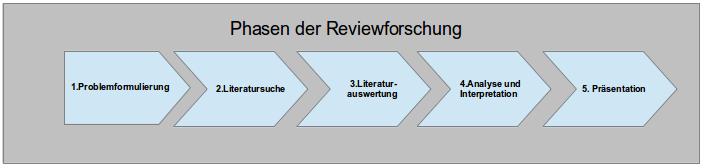
\includegraphics[width=1\linewidth]{Bilder/phasen.png}
	\captionof{figure}[Fünf Phasen der Reviewforschung]
	\label{Fünf Phasen der Reviewforschung}
\end{minipage}

Wärend der ersten Phase wird die Frage, die durch das Review zu beantworten
ist präzise ausformuliert. Das auswerten der Literatur ist in der zweiten Phase beschrieben. Darin geht es Primär darum für die Fragestellung geeignete Literatur zu recherchieren. Darauf folgt die Identifizierung von Relevanter Literatur welche man dann in der vierten Phase Analysiert und Interpretiert. Das Präsentieren der Ergebnisse ist die letzte der fünf Phasen.Für diese Analyse werden Primär Quellen in spezialisierte Suchmaschinen für wissenschaftlich Publikationen gesucht. Während der Untersuchung und Ausarbeitung dieser Analyse wurden ausschließlich folgende
Suchmaschinen genutzt.
\begin{compactitem}
	\item link.springer.com
	\item scholar.google.de
	\item boss.bsz-bw.de/HSHN/
\end{compactitem}
zur auswahl der in dieser Arbeit benutzten wissenschaftlichen Zeitschriften  gehören die vom Springer-Verlag herausgegebene Zeitschrift Informatik Spektrum sowie die Zeitschrift Wirtschaftsinformatik sowie "Journal of management information systems". Diese Zeitschriften sind auf der WI-Journalliste 2008 zu finden. Diese Liste soll als Orientierung dienen. Ausgearbeitet von  zwei Arbeitskreisen deren Mitglieder universitets Professoren aus Österreich, Deutschland und der Schweiz sind\cite{WiLis}.Um zu verdeutlichen welche Herausforderungen in der Praxis existieren werden auch Artikel aus der Fachzeitschrift Controlling & Management und die Untersuchung miteinbezogen.
Der zeitlichen Intervall zur Auswahl der Literatur wird auf 1990 bis 2014. Weil seit Mitte der 1990er Jahre Systeme, in einem Unternehmen zur Entscheidungsfindung herangezogen werden.\footnote{\cite{Humm}} Für der Art von Entscheidungen ist eine hohe Datenqualität von enormer Wichtigkeit. Da her lässt sich In dieser Zeitspanne kurz vor beginn der Nutzung Entscheidungsunterstüzender Systeme bis heute Relevante Litaratur finden.

Die Keywords welche zur Recherche in den oben genannten Suchmaschinen genutzt werden sind dem Kontext des Fachbereichs einzuordnen.

Keywords Rubrik Datenqualität
\begin{compactitem}
	\item --Datenqualität - data quality
	\item --Data Governance 
\end{compactitem}

Keywords Rubrik Technik \& Architektur
\begin{compactitem}
	\item --Data Warehouse 
	\item --Datenbankmanagementsystem 
	\item --Daten bereinigung - Data cleaning
\end{compactitem}

Keywords Rubrik Informationsmanagement und Organisation
\begin{compactitem}
	\item Informationsmanagement 
	\item Datenqualitätsmanagement
\end{compactitem}


Die Suchbegriffe sind den Rubriken zuzuordnen, für die Datenqualität sowie Data Governance unter der Rubrik Datenqualität gilt es zu Untersuchen welche Definitionen und Ansätze es bereits gibt.Der Begriff Data Warehouse soll aufzeigen ob Unterschiede in der Modellierung sowie der Architektur eines Systems Einfluss auf die Datenqualität haben. Datenbankmanagementsystem als Suchbegriff
soll Klarheit schaffen ob die Wahl des DMS eine Rolle hinsichtlich der Datenqualität spielt. Aber auch das Bereinigen von Daten soll untersucht werden um Nachhaltigkeit zu gewährleisten.
Die Rubrik Informationsmanagement und Organisation soll den Faktor Mensch Repräsentieren, und aufzeigen in wie weit Datenqualität abhängig vom Menschen ist.  
\newpage
\subsection{Suchprotokoll}
Der Suchbegriff Datenqualität ergab 10 Ergebnisse wobei die suche durch Angabe des Zeitintervalls von 1990 bis 2014 und nur im Titel gefiltert wurde. Diese sind soweit als Grundeinstellung für jede weitere suche bei Springerlink zu sehen. Datenqualitätsmanagement ergab 16 Treffer, 17 Artikel wurden bei dem Suchbegriff Datenbankmanagementsystem angezeigt. Weiter suchen ergaben folgendes:


\vspace{1em}
\begin{table}[!h]
	\centering
	\begin{tabular}{|l|l|l|}
		\hline
		\textbf{Suchbegriff} & \textbf{Anzahl} & \textbf{Suchmaschine}\\
		\hline
		Data Governance & 1 & Springerlink\\
		\hline
		Data Warehouse
 & 7 & Springerlink\\
		\hline
		Datenbereinigung  & 32 & Springerlink\\
		\hline
		
		Informationsmanagement  & 15 & Springerlink\\
		\hline
	\end{tabular}
	\caption{Beispieltabelle}
	\label{tab:beispiel}
\end{table}

Es werden nur Publikationen berücksichtigt welche Beschreiben wie Qualität der Daten verbessert werden kann.

  
\section{Faktor Datenqualität}
Die Qualität von Daten wird von verschiedensten Faktoren bestimmt,  laut Redman die Fähigkeit, die Anforderungen der beabsichtigten
Nutzung in einer bestimmten Situation zu erfüllen („fitness for use“) \cite{redman} in Kombination mit den Qualitätsmerkmalen nach Wang & Strong, welche die Merkmale Klassifizieren und somit Redmans Definition stützen. 

\section{Technische Faktoren}
\section{Faktor Organisation}

\subsection{Bilder}
Zum Einfügen eines Bildes, siehe Abbildung \ref{fig:osgi}, wird die \textit{minipage}-Umgebung genutzt, da die Bilder so gut positioniert werden können.

\vspace{1em}
\begin{minipage}{\linewidth}
	\centering
	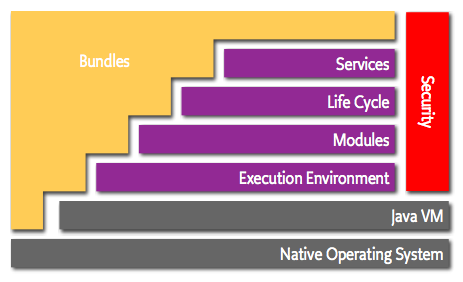
\includegraphics[width=0.7\linewidth]{Bilder/layering-osgi.png}
	\captionof{figure}[OSGi Architektur]{OSGi Architektur\footnotemark }
	\label{fig:osgi}
\end{minipage}
\footnotetext{Quelle: \url{http://www.osgi.org/Technology/WhatIsOSGi}}

\subsection{Tabellen}
In diesem Abschnitt wird eine Tabelle (siehe Tabelle \ref{tab:beispiel}) dargestellt.

\vspace{1em}
\begin{table}[!h]
	\centering
	\begin{tabular}{|l|l|l|}
		\hline
		\textbf{Name} & \textbf{Name} & \textbf{Name}\\
		\hline
		1 & 2 & 3\\
		\hline
		4 & 5 & 6\\
		\hline
		7 & 8 & 9\\
		\hline
	\end{tabular}
	\caption{Beispieltabelle}
	\label{tab:beispiel}
\end{table}

\pagebreak
\subsection{Auflistung}
Für Auflistungen wird die \textit{compactitem}-Umgebung genutzt, wodurch der Zeilenabstand zwischen den Punkten verringert wird.

\begin{compactitem}
	\item Nur
	\item ein
	\item Beispiel.
\end{compactitem}

\subsection{Listings}
Zuletzt ein Beispiel für ein Listing, in dem Quellcode eingebunden werden kann, siehe Listing \ref{lst:arduino}.

\vspace{1em}
\begin{lstlisting}[caption=Arduino Beispielprogramm, label=lst:arduino]
int ledPin = 13;
void setup() {
    pinMode(ledPin, OUTPUT);
}
void loop() {
    digitalWrite(ledPin, HIGH);
    delay(500);
    digitalWrite(ledPin, LOW);
    delay(500);
}
\end{lstlisting}

\subsection{Tipps}
Die Quellen befinden sich in der Datei \textit{bibo.bib}. Ein Buch- und eine Online-Quelle sind beispielhaft eingefügt. [Vgl. \cite{buch}, \cite{online}]

Abkürzungen lassen sich natürlich auch nutzen (\ac{OSGi}). Weiter oben im Latex-Code findet sich das Verzeichnis.
\pagebreak

% ----------------------------------------------------------------------------------------------------------
% Kapitel
% ----------------------------------------------------------------------------------------------------------
\section{Kapitel}
Lorem ipsum dolor sit amet.

\subsection{Unterkapitel}
Lorem ipsum dolor sit amet, consetetur sadipscing elitr, sed diam nonumy eirmod tempor invidunt ut labore et dolore magna aliquyam erat, sed diam voluptua. At vero eos et accusam et justo duo dolores et ea rebum. Stet clita kasd gubergren, no sea takimata sanctus est Lorem ipsum dolor sit amet. Lorem ipsum dolor sit amet, consetetur sadipscing elitr, sed diam nonumy eirmod tempor invidunt ut labore et dolore magna aliquyam erat, sed diam voluptua. At vero eos et accusam et justo duo dolores et ea rebum. Stet clita kasd gubergren, no sea takimata sanctus est Lorem ipsum dolor sit amet.

\subsection{Unterkapitel}
Lorem ipsum dolor sit amet, consetetur sadipscing elitr, sed diam nonumy eirmod tempor invidunt ut labore et dolore magna aliquyam erat, sed diam voluptua. At vero eos et accusam et justo duo dolores et ea rebum. Stet clita kasd gubergren, no sea takimata sanctus est Lorem ipsum dolor sit amet. Lorem ipsum dolor sit amet, consetetur sadipscing elitr, sed diam nonumy eirmod tempor invidunt ut labore et dolore magna aliquyam erat, sed diam voluptua. At vero eos et accusam et justo duo dolores et ea rebum. Stet clita kasd gubergren, no sea takimata sanctus est Lorem ipsum dolor sit amet.
\pagebreak

% ----------------------------------------------------------------------------------------------------------
% Kapitel
% ----------------------------------------------------------------------------------------------------------
\section{Kapitel}
Lorem ipsum dolor sit amet.

\subsection{Unterkapitel}
Lorem ipsum dolor sit amet, consetetur sadipscing elitr, sed diam nonumy eirmod tempor invidunt ut labore et dolore magna aliquyam erat, sed diam voluptua. At vero eos et accusam et justo duo dolores et ea rebum. Stet clita kasd gubergren, no sea takimata sanctus est Lorem ipsum dolor sit amet. Lorem ipsum dolor sit amet, consetetur sadipscing elitr, sed diam nonumy eirmod tempor invidunt ut labore et dolore magna aliquyam erat, sed diam voluptua. At vero eos et accusam et justo duo dolores et ea rebum. Stet clita kasd gubergren, no sea takimata sanctus est Lorem ipsum dolor sit amet.

\subsection{Unterkapitel}
Lorem ipsum dolor sit amet, consetetur sadipscing elitr, sed diam nonumy eirmod tempor invidunt ut labore et dolore magna aliquyam erat, sed diam voluptua. At vero eos et accusam et justo duo dolores et ea rebum. Stet clita kasd gubergren, no sea takimata sanctus est Lorem ipsum dolor sit amet. Lorem ipsum dolor sit amet, consetetur sadipscing elitr, sed diam nonumy eirmod tempor invidunt ut labore et dolore magna aliquyam erat, sed diam voluptua. At vero eos et accusam et justo duo dolores et ea rebum. Stet clita kasd gubergren, no sea takimata sanctus est Lorem ipsum dolor sit amet.
\pagebreak

% ----------------------------------------------------------------------------------------------------------
% Kapitel
% ----------------------------------------------------------------------------------------------------------
\section{Kapitel}
Lorem ipsum dolor sit amet.

\subsection{Unterkapitel}
Lorem ipsum dolor sit amet, consetetur sadipscing elitr, sed diam nonumy eirmod tempor invidunt ut labore et dolore magna aliquyam erat, sed diam voluptua. At vero eos et accusam et justo duo dolores et ea rebum. Stet clita kasd gubergren, no sea takimata sanctus est Lorem ipsum dolor sit amet. Lorem ipsum dolor sit amet, consetetur sadipscing elitr, sed diam nonumy eirmod tempor invidunt ut labore et dolore magna aliquyam erat, sed diam voluptua. At vero eos et accusam et justo duo dolores et ea rebum. Stet clita kasd gubergren, no sea takimata sanctus est Lorem ipsum dolor sit amet.

\subsection{Unterkapitel}
Lorem ipsum dolor sit amet, consetetur sadipscing elitr, sed diam nonumy eirmod tempor invidunt ut labore et dolore magna aliquyam erat, sed diam voluptua. At vero eos et accusam et justo duo dolores et ea rebum. Stet clita kasd gubergren, no sea takimata sanctus est Lorem ipsum dolor sit amet. Lorem ipsum dolor sit amet, consetetur sadipscing elitr, sed diam nonumy eirmod tempor invidunt ut labore et dolore magna aliquyam erat, sed diam voluptua. At vero eos et accusam et justo duo dolores et ea rebum. Stet clita kasd gubergren, no sea takimata sanctus est Lorem ipsum dolor sit amet.
\pagebreak

% ----------------------------------------------------------------------------------------------------------
% Literatur
% ----------------------------------------------------------------------------------------------------------
\renewcommand\refname{Quellenverzeichnis}
\bibliographystyle{myalpha}
\bibliography{bibo}
\pagebreak

% ----------------------------------------------------------------------------------------------------------
% Anhang
% ----------------------------------------------------------------------------------------------------------
\pagenumbering{Roman}
\setcounter{page}{1}
\lhead{Anhang \thesection}

\begin{appendix}
\section*{Anhang}
\phantomsection
\addcontentsline{toc}{section}{Anhang}
\addtocontents{toc}{\vspace{-0.5em}}

\section{GUI}
Ein toller Anhang.

\subsection*{Screenshot}
\label{app:screenshot}
Unterkategorie, die nicht im Inhaltsverzeichnis auftaucht.

\end{appendix}


\newpage
\thispagestyle{empty}
\begin{center}
	\vspace*{5em}
	\huge\textbf{Erklärung}\\
\end{center}
\vspace{2em}
Hiermit versichere ich, dass ich meine Abschlussarbeit selbständig verfasst und keine anderen als die angegebenen Quellen und Hilfsmittel benutzt habe.

\vspace{4em}
\begin{minipage}{\linewidth}
	\begin{tabular}{p{15em}p{15em}}
		Datum: &  .......................................................\\
		& \centering (Unterschrift)\\
	\end{tabular}
\end{minipage}

\end{document}
